%%%%%%%%%%%%%%%%%%%%%%%%%%%%%%%%%%%%%%%%%%%%%%
%
%		Thesis Settings
%
%		EDOC Template
%		2011
%
%%%%%%%%%%%%%%%%%%%%%%%%%%%%%%%%%%%%%%%%%%%%%%
\documentclass[a4paper,11pt,fleqn]{article}

\usepackage[T1]{fontenc}
\usepackage[utf8]{inputenc}
\usepackage[french,german,english]{babel}


%%%%%%%%%%%%%%%%%%%%%%%%%%%%%%%%%%%%%%%%%%%%%%%
%% EDOC THESIS TEMPLATE: Variant 1.0 -> Latin modern, large text width&height
%%%%%%%%%%%%%%%%%%%%%%%%%%%%%%%%%%%%%%%%%%%%%%%
%\usepackage{lmodern}
%\usepackage[a4paper,top=22mm,bottom=28mm,inner=35mm,outer=25mm]{geometry}
%%%%%%%%%%%%%%%%%%%%%%%%%%%%%%%%%%%%%%%%%%%%%%%

%%%%%%%%%%%%%%%%%%%%%%%%%%%%%%%%%%%%%%%%%%%%%%
% EDOC THESIS TEMPLATE: Variant 2.0 -> Utopia, Gabarrit A (lighter pages)
%%%%%%%%%%%%%%%%%%%%%%%%%%%%%%%%%%%%%%%%%%%%%%
\usepackage{fourier} % Utopia font-typesetting including mathematical formula compatible with newer TeX-Distributions (>2010)
%\usepackage{utopia} % on older systems -> use this package instead of fourier in combination with mathdesign for better looking results
%\usepackage[adobe-utopia]{mathdesign}
\setlength{\textwidth}{146.8mm} % = 210mm - 37mm - 26.2mm
\setlength{\oddsidemargin}{11.6mm} % 37mm - 1in (from hoffset)
\setlength{\evensidemargin}{0.8mm} % = 26.2mm - 1in (from hoffset)
\setlength{\topmargin}{-2.2mm} % = 0mm -1in + 23.2mm
\setlength{\textheight}{221.9mm} % = 297mm -29.5mm -31.6mm - 14mm (12 to accomodate footline with pagenumber)
\setlength{\headheight}{14pt}
%%%%%%%%%%%%%%%%%%%%%%%%%%%%%%%%%%%%%%%%%%%%%%



\setlength{\parindent}{0pt}

\usepackage{setspace} % increase interline spacing slightly
\setstretch{1.1}

\makeatletter
\setlength{\@fptop}{0pt}  % for aligning all floating figures/tables etc... to the top margin
\makeatother


\usepackage{graphicx,xcolor}
\graphicspath{{images/}}

\usepackage{subfig}
\usepackage{booktabs}
\usepackage{lipsum}
\usepackage{microtype}
\usepackage{url}
\usepackage[final]{pdfpages}

\usepackage{fancyhdr}
\renewcommand{\sectionmark}[1]{\markright{\thesection\ #1}}
\pagestyle{fancy}
	\fancyhf{}
	\renewcommand{\headrulewidth}{0.4pt}
	\renewcommand{\footrulewidth}{0pt}
	\fancyhead[OR]{\bfseries \nouppercase{\rightmark}}
	\fancyhead[EL]{\bfseries \nouppercase{\leftmark}}
	\fancyfoot[EL,OR]{\thepage}
\fancypagestyle{plain}{
	\fancyhf{}
	\renewcommand{\headrulewidth}{0pt}
	\renewcommand{\footrulewidth}{0pt}
	\fancyfoot[EL,OR]{\thepage}}
\fancypagestyle{addpagenumbersforpdfimports}{
	\fancyhead{}
	\renewcommand{\headrulewidth}{0pt}
	\fancyfoot{}
	\fancyfoot[RO,LE]{\thepage}
}

\usepackage{listings}
\lstset{language=[LaTeX]Tex,tabsize=4, basicstyle=\scriptsize\ttfamily, showstringspaces=false, numbers=left, numberstyle=\tiny, numbersep=10pt, breaklines=true, breakautoindent=true, breakindent=10pt}

\usepackage{hyperref}
\hypersetup{pdfborder={0 0 0},
	colorlinks=true,
	linkcolor=black,
	citecolor=black,
	urlcolor=black}
\urlstyle{same}

\makeatletter
\def\cleardoublepage{\clearpage\if@twoside \ifodd\c@page\else
    \hbox{}
    \thispagestyle{empty}
    \newpage
    \if@twocolumn\hbox{}\newpage\fi\fi\fi}
\makeatother \clearpage{\pagestyle{plain}\cleardoublepage}


%%%%% CHAPTER HEADER %%%%
\usepackage{color}
\usepackage{tikz}
\usepackage[explicit]{titlesec}
\newcommand*\chapterlabel{}
%\renewcommand{\thechapter}{\Roman{chapter}}
\titleformat{\chapter}[display]  % type (section,chapter,etc...) to vary,  shape (eg display-type)
	{\normalfont\bfseries\Huge} % format of the chapter
	{\gdef\chapterlabel{\thechapter\ }}     % the label
 	{0pt} % separation between label and chapter-title
 	  {\begin{tikzpicture}[remember picture,overlay]
    \node[yshift=-8cm] at (current page.north west)
      {\begin{tikzpicture}[remember picture, overlay]
        \draw[fill=black] (0,0) rectangle(35.5mm,15mm);
        \node[anchor=north east,yshift=-7.2cm,xshift=34mm,minimum height=30mm,inner sep=0mm] at (current page.north west)
        {\parbox[top][30mm][t]{15mm}{\raggedleft $\phantom{\textrm{l}}$\color{white}\chapterlabel}};  %the black l is just to get better base-line alingement
        \node[anchor=north west,yshift=-7.2cm,xshift=37mm,text width=\textwidth,minimum height=30mm,inner sep=0mm] at (current page.north west)
              {\parbox[top][30mm][t]{\textwidth}{\color{black}#1}};
       \end{tikzpicture}
      };
   \end{tikzpicture}
   \gdef\chapterlabel{}
  } % code before the title body

\titlespacing*{\chapter}{0pt}{50pt}{30pt}
\titlespacing*{\section}{0pt}{13.2pt}{*0}  % 13.2pt is line spacing for a text with 11pt font size
\titlespacing*{\subsection}{0pt}{13.2pt}{*0}
\titlespacing*{\subsubsection}{0pt}{13.2pt}{*0}

\newcounter{myparts}
\newcommand*\partlabel{}
\titleformat{\part}[display]  % type (section,chapter,etc...) to vary,  shape (eg display-type)
	{\normalfont\bfseries\Huge} % format of the part
	{\gdef\partlabel{\thepart\ }}     % the label
 	{0pt} % separation between label and part-title
 	  {\setlength{\unitlength}{20mm}
	  \addtocounter{myparts}{1}
	  \begin{tikzpicture}[remember picture,overlay]
    \node[anchor=north west,xshift=-65mm,yshift=-6.9cm-\value{myparts}*20mm] at (current page.north east) % for unknown reasons: 3mm missing -> 65 instead of 62
      {\begin{tikzpicture}[remember picture, overlay]
        \draw[fill=black] (0,0) rectangle(62mm,20mm);   % -\value{myparts}\unitlength
        \node[anchor=north west,yshift=-6.1cm-\value{myparts}*20mm,xshift=-60.5mm,minimum height=30mm,inner sep=0mm] at (current page.north east)
        {\parbox[top][30mm][t]{55mm}{\raggedright \color{white}Part \partlabel $\phantom{\textrm{l}}$}};  %the phantom l is just to get better base-line alingement
        \node[anchor=north east,yshift=-6.1cm-\value{myparts}*20mm,xshift=-63.5mm,text width=\textwidth,minimum height=30mm,inner sep=0mm] at (current page.north east)
              {\parbox[top][30mm][t]{\textwidth}{\raggedleft \color{black}#1}};
       \end{tikzpicture}
      };
   \end{tikzpicture}
   \gdef\partlabel{}
  } % code before the title body

\usepackage{amsmath}
% Fix the problem with delimiter size caused by fourier and amsmath packages.
\makeatletter
\def\resetMathstrut@{%
  \setbox\z@\hbox{%
    \mathchardef\@tempa\mathcode`\(\relax
      \def\@tempb##1"##2##3{\the\textfont"##3\char"}%
      \expandafter\@tempb\meaning\@tempa \relax
  }%
  \ht\Mathstrutbox@1.2\ht\z@ \dp\Mathstrutbox@1.2\dp\z@
}
\makeatother

\usepackage{pbox}
\usepackage{tabularx}
\usepackage{wrapfig}
\usepackage{csvsimple}
\usepackage{paralist}
\usepackage{csquotes}

\definecolor{red}{rgb}{1,0,0}
\newcommand{\fix}[1]{\textbf{\color{red}{#1}}}
\newcommand{\fig}[1]{Figure~\ref{#1}}
\newcommand{\sref}[1]{Section~\ref{#1}}
\newcommand{\aref}[1]{Appendix~\ref{#1}}
\clubpenalty=10000
\widowpenalty=10000

\begin{document}
\begin{titlepage}
\begin{center}
\sffamily
\null\vspace{2cm}
{\huge Modern Distributed Rendering Systems\par}
\vfill
\begin{tabular}{cc}
\parbox{0.4\textwidth}{
\includegraphics[width=5cm]{images/uzh}}
&
\parbox{0.6\textwidth}{%
        Dissertation\\
        Submitted TBD\\[9pt]
        to the Faculty of Economics, Business Administration and Information Technology of the University of Z\"urich\\[9pt]
        for the degree of\\
        Doctor of Science (Ph.D)\\[9pt]
        by Stefan Eilemann\\[9pt]
        Supervisor: Prof. Dr. Renato Pajarola\\
        Co-referee: TBD}
\end{tabular}
\end{center}
\vspace{2cm}
\end{titlepage}
\setcounter{page}{0}

\section*{Abstract}
We are living in the big data age: An ever increasing amount of data is being
produced by users through data acquisition and simulations. While large scale
analysis and simulatons have received significant attention for cloud computing
and HPC systems, software to efficiently visualize large amounts of data is
struggling to keep up.

We propose to research system software to facilitate and accelerate large data
visualization through parallel rendering, and to validate the research and
development of this system software by the development of new applications for
large data visualization.

This research and development will enable domain scientists and large data
engineers to better extract meaning from their data, making it feasible to
explore more data by accelerating the rendering and allowing the use of
high-resolution displays to see more detail.

Due to the nature of this research, we propose an engineering-driven, iterative
research process. Based on the foundations of a generic parallel rendering
system, individual research questions can be addressed in isolation and
optimized through data-driven benchmarking, and integrated in product quality
into the parallel rendering system.

\vfill

\section*{Acknowledgements}

The research leading to this proposal was supported in part by the Blue Brain
Project, the Swiss National Science Foundation under Grant 200020-129525, the
European Union Seventh Framework Programme (FP7/2007-2013) under grant agreement
no. 604102 (Human Brain Project), the Hasler Stiftung grant (project number
$12097$), and the King Abdullah University of Science and Technology (KAUST)
through the KAUST-EPFL alliance for Neuro-Inspired High Performance Computing.

I would like to take the opportunity to thank the Blue Brain Project, in
particular the visualization team, and all the other contributors for their
support in the research leading to this proposal. Furthermore, I would like to
thank Prof. Renato Pajarola for his long-term commitment to my research work.

\bigskip
\noindent\textit{Neuch\^atel, \today}
\hfill Stefan Eilemann
\clearpage

% \tableofcontents
% \listoffigures
% \listoftables

\setlength{\parskip}{1em}

\section{Motivation} % 1-2 pages

After decades of exponential growth in computational performance, storage and
data acquisition, computing is now well in the big data age, where future
advances are measured in our capability to extract meaningful information from
the available data. Visual analysis based on interactive rendering of
three-dimensional data has been proven to be a particularly efficient approach
to gain intuitive insight into the spatial structure and relations of very large
3D data sets. These developments create new, unique challenges for applications
and system software to enable users to fully exploit the available resources to
gain insight from their data.

The quantity of computed, measured or collected data is exponentially growing,
fueled by the pervasive diffusion of digitalization in modern life. Moreover,
the fields of science, engineering and technology are increasingly defined by a
data driven approach to conduct research and development. High-quality and
large-scale data is continuously generated at a growing rate from sensor and
scanning systems, as well as from data collections and numerical simulations in
a number of science and technology domains.

\begin{figure}[ht]\label{FIG_teaser}
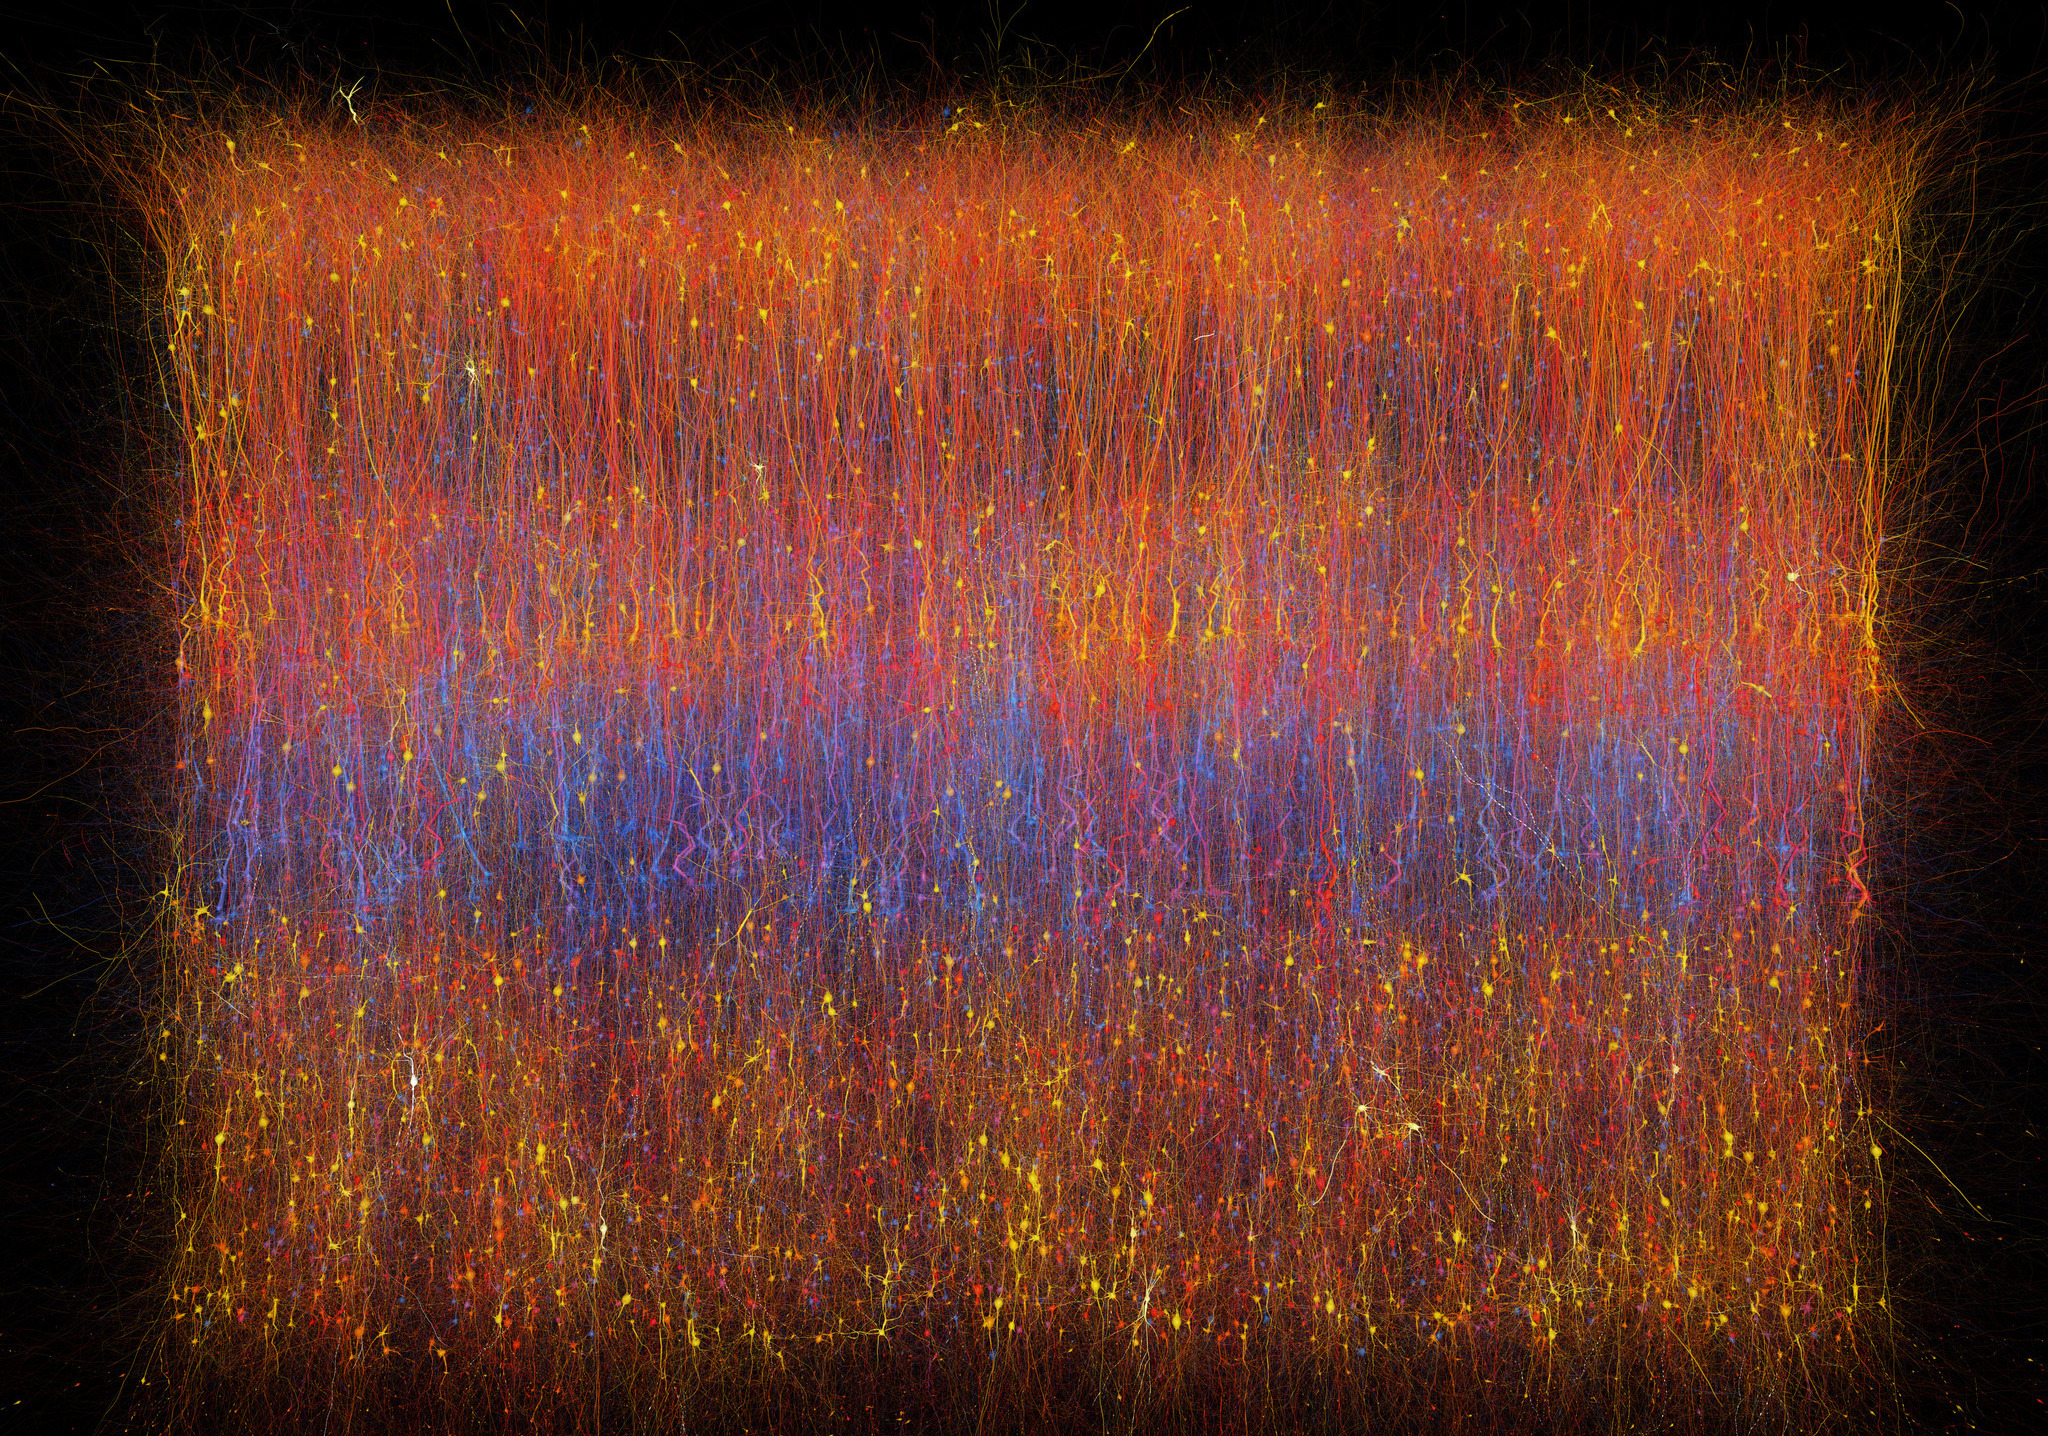
\includegraphics[height=5cm]{images/slices}\hfil%
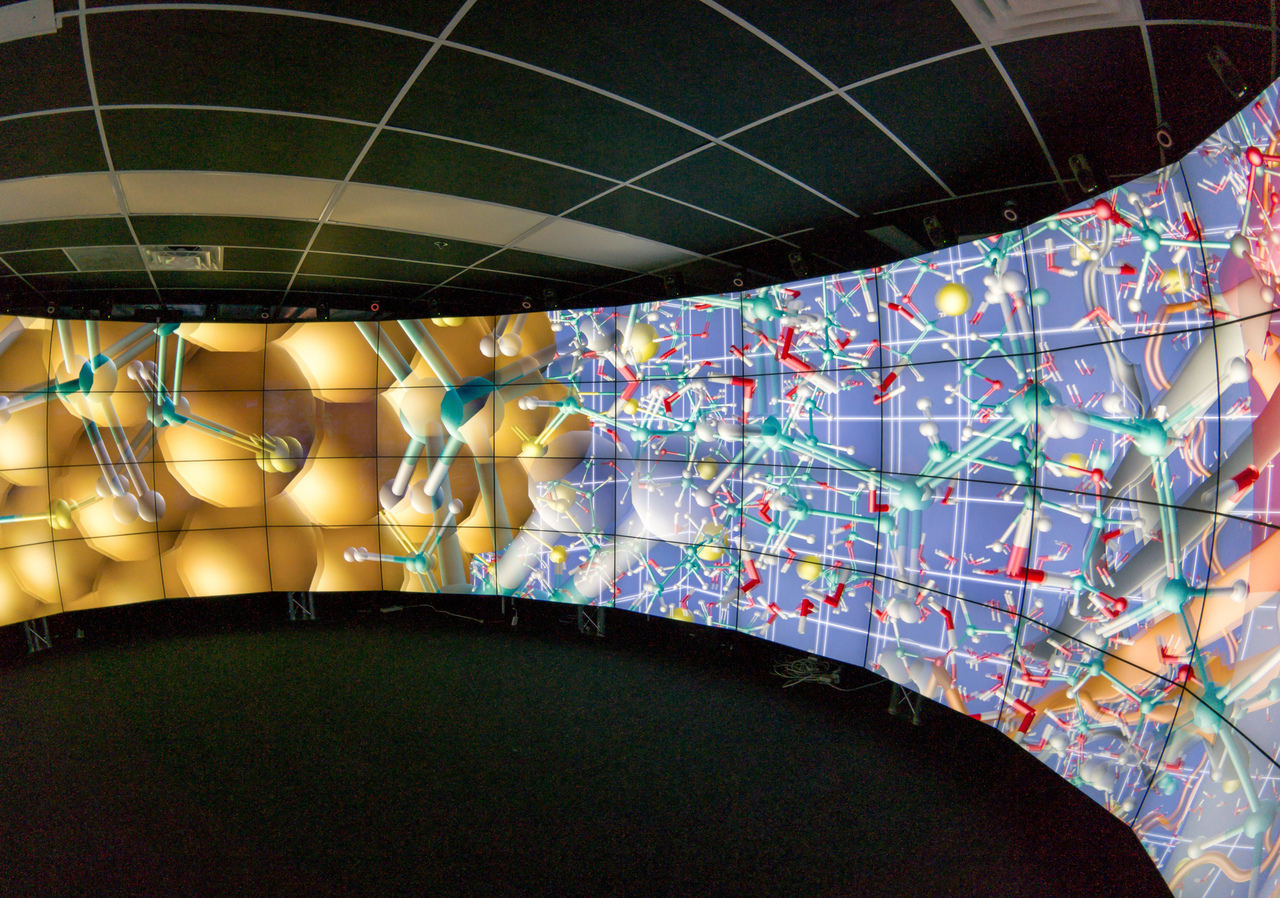
\includegraphics[height=5cm]{images/cave2}\\%
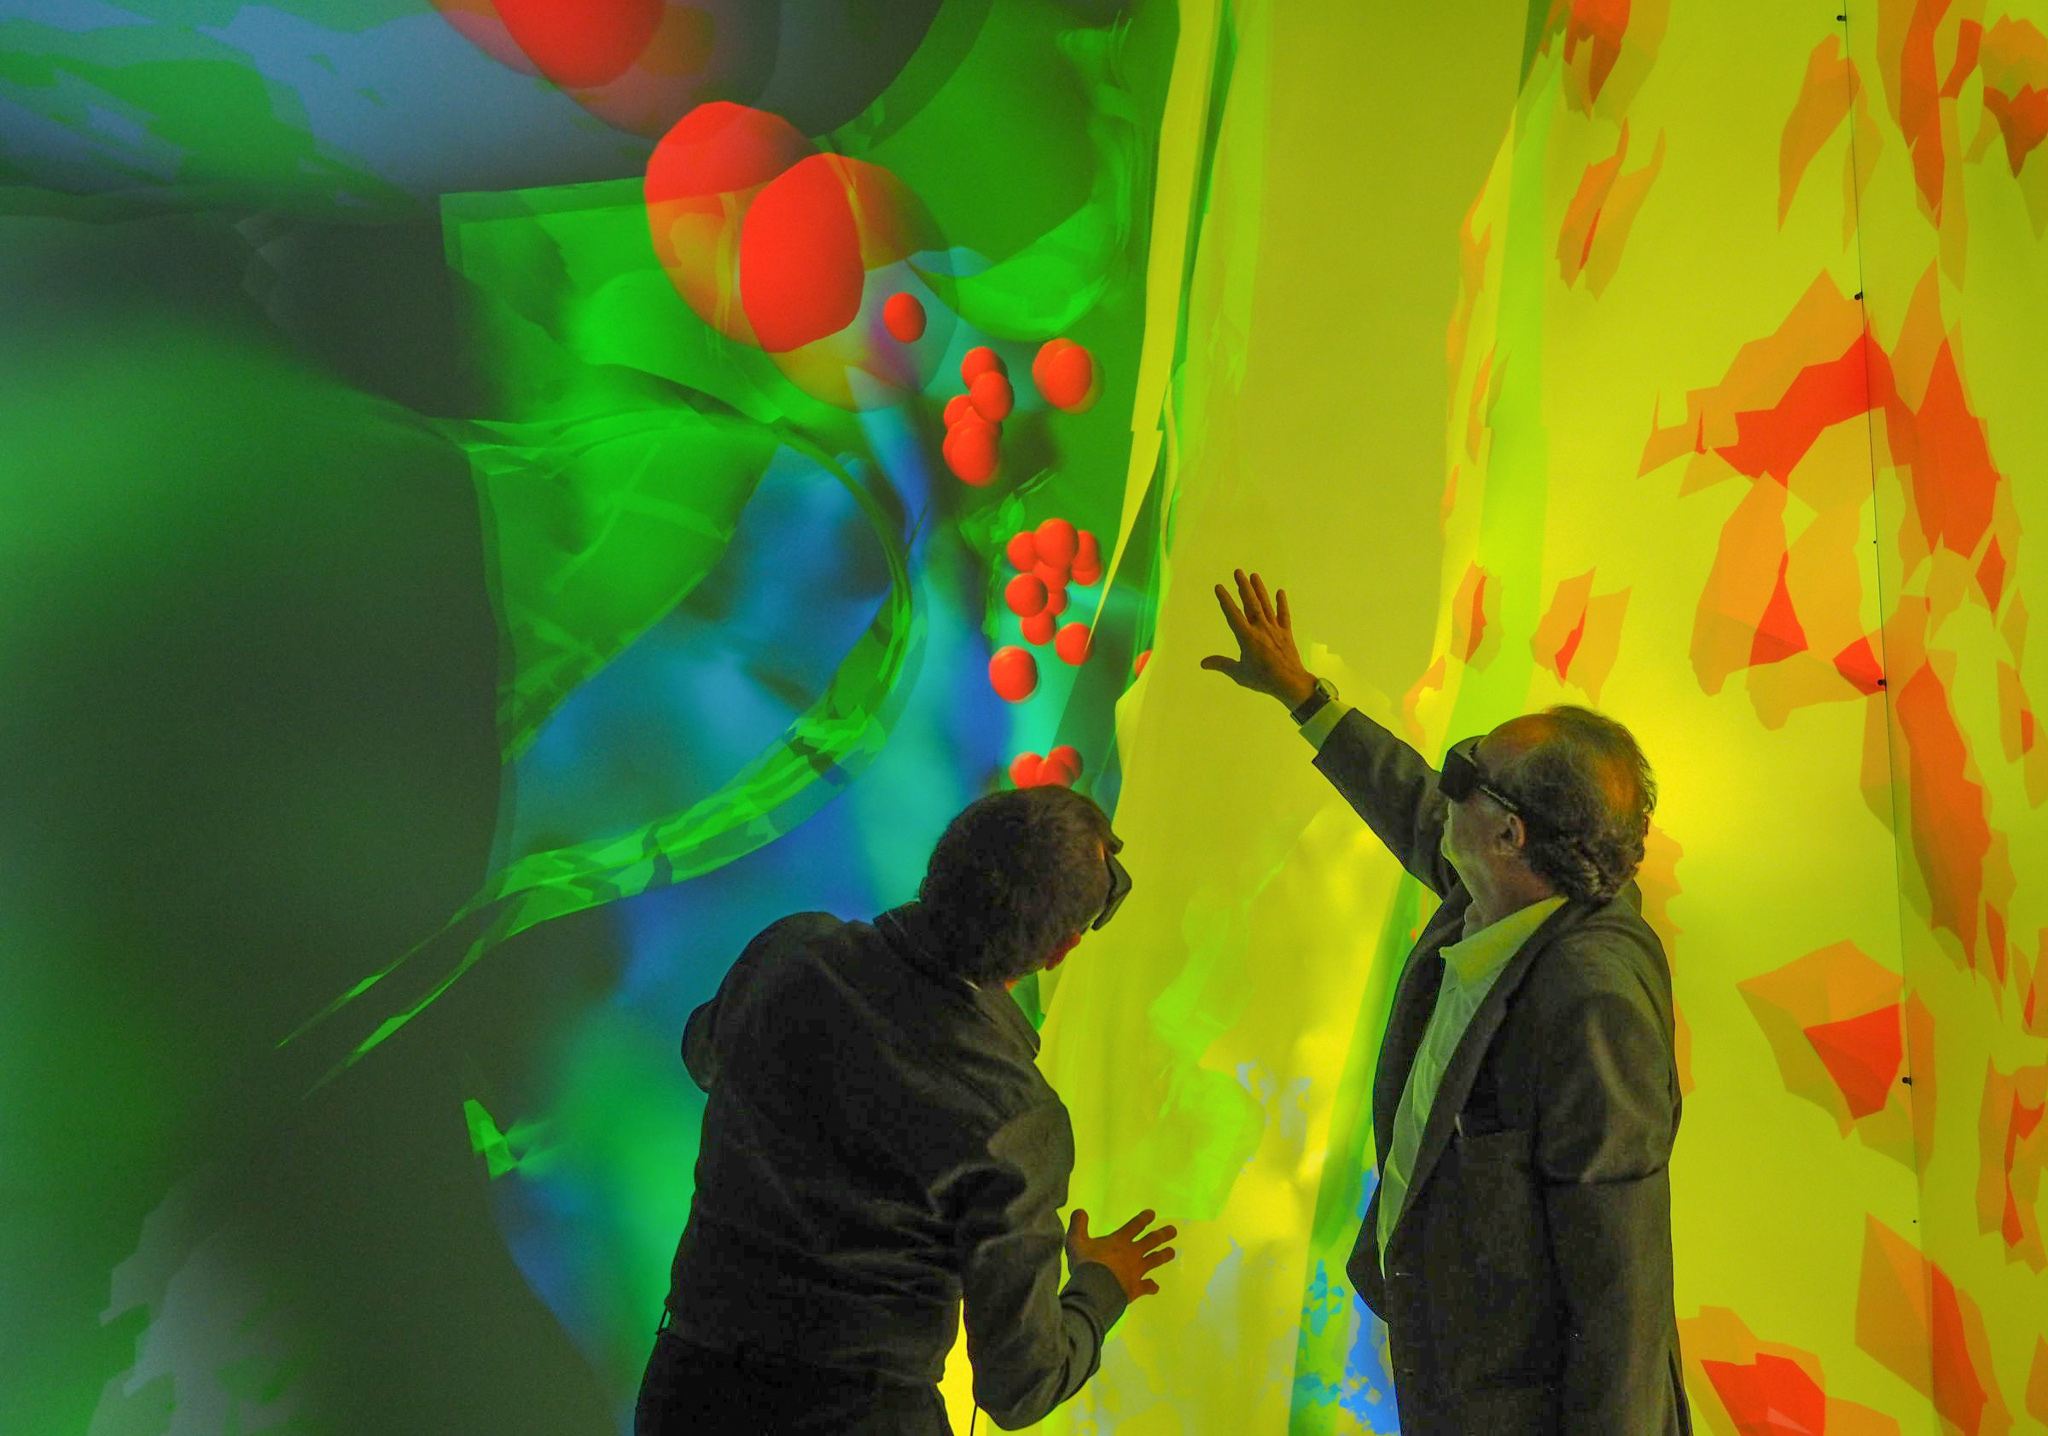
\includegraphics[height=5.27cm]{images/cave}\hfil%
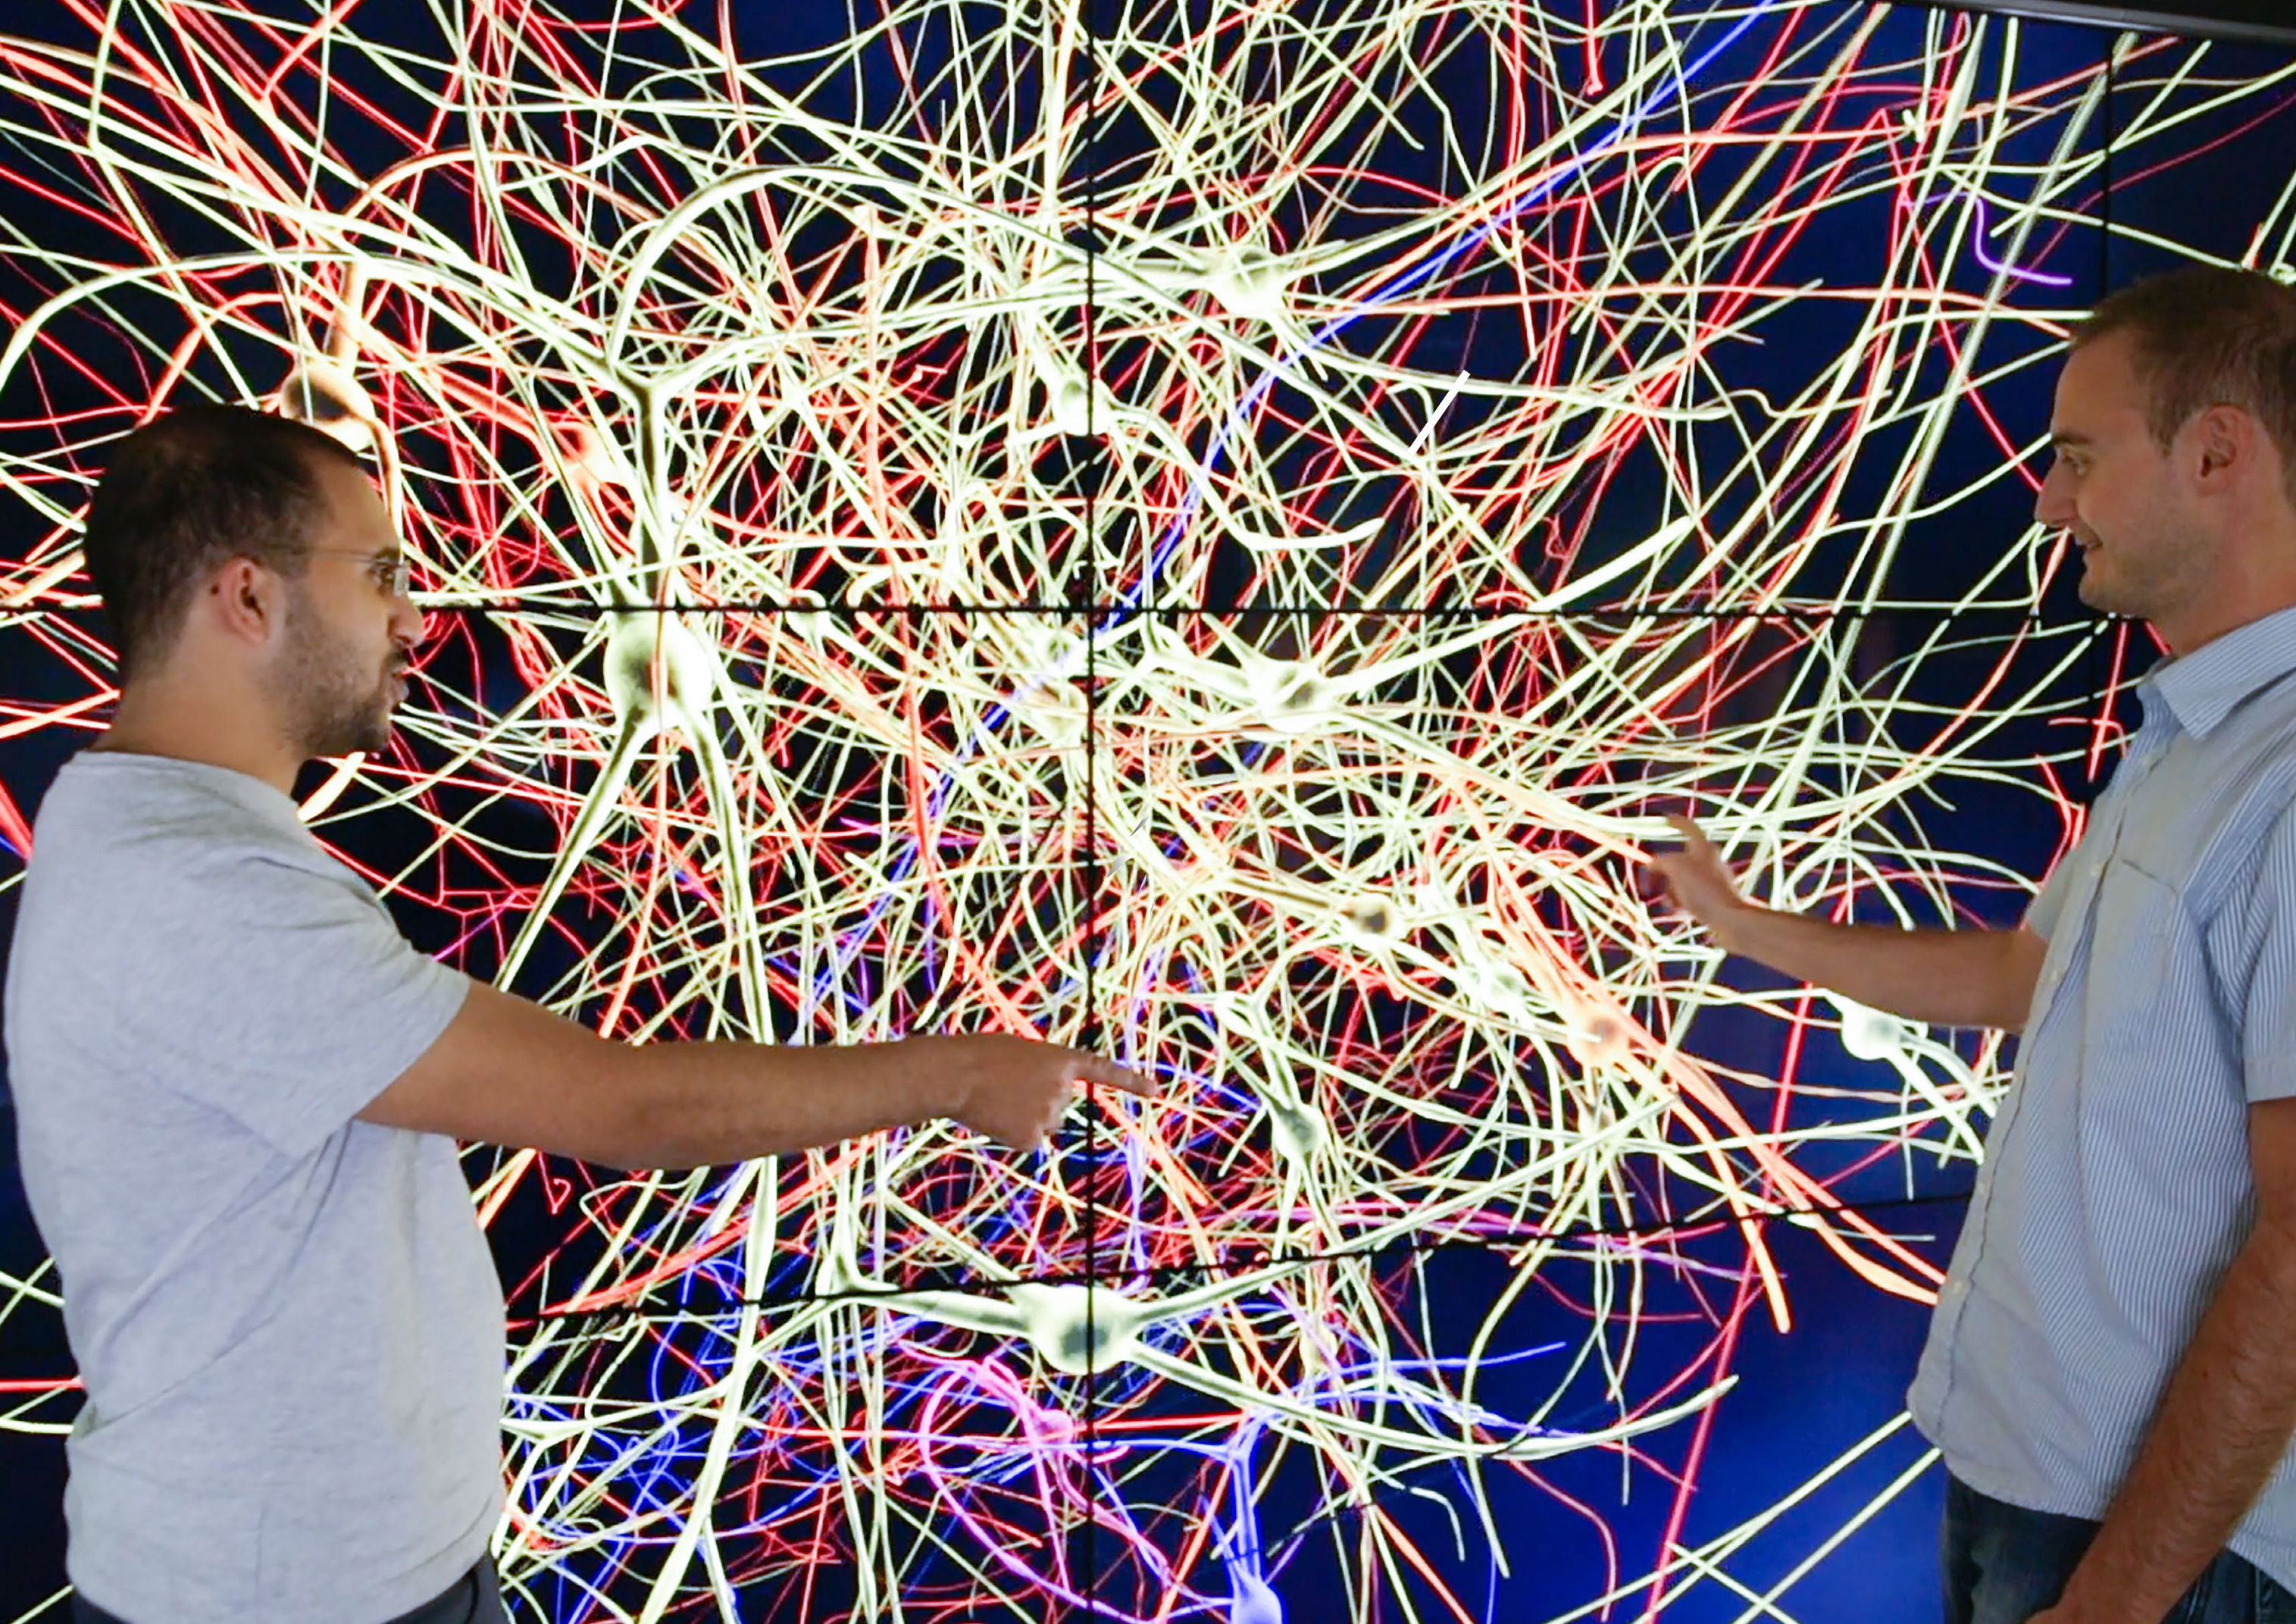
\includegraphics[height=5.27cm]{images/tide}%
\caption{Large Data Visualization: Large data visualization of a
      brain simulation, molecular visualization in the Cave$^2$, exploration of EM
      stack reconstructions in a Cave, collaborative data analysis on a tiled
      display wall.}
\end{figure}

Display technology has made significant progress in the last decade.
High-resolution screens and tiled display walls are now affordabe for most
organizations and are getting deployed at an increasing rate. This increased
resolution and display size helps with understanding the data, but with the
quadratic increase in pixels to be rendered, it increases the pressure on
rendering algorithms to deliver interactive framerates. Furthermore, for larger
system it becomes necessary to develop parallel and distributed applications.

However, not only applications are becoming more and more data-driven, but also
the technology used to tackle these kinds of problems is rapidly witnessing a
paradigm shift towards massively parallel on-chip and distributed parallel
cluster solutions. On one hand, parallelism within a system has increased
massively, with tenths of CPU cores, thousands of GPU cores and multiple CPUs
and GPUs in a single system. On the other hand, massively parallel distributed
systems are easily accessible from various cloud infrastructure providers, and
are also affordable for on-site hosting for many organizations.

System software to exploit the available hardware parallelism capable of
performing efficient interactive data exploration has not kept up with the pace
in hardware developments and data gathering capabilities. On one hand, this is
due to an inherent delay between hardware and software capabilities, since
development typically only starts once the hardware is available. On the other
hand, existing software engineered for different design parameters has a
significant inertia to change, to the extreme of the necessity to rewrite it
from scratch.

In the context of emerging data-intensive knowledge discovery and data analysis,
efficient interactive data exploration methodologies have become increasingly
important. Visual analysis by means of interactive visualization and inspection
of three-dimensional data is a particularly efficient approach to gain intuitive
insight into the spatial structure and relations of very large 3D data sets.
However, defining visual and interactive methods scalable with problem size and
degree of parallelism, as well as generic applicability of high-performance
interactive visualization methods and systems are recognized among the major
current and future challenges.


\section{Related Work} % 2-6

The main performance indicator for Large Data Interactive Rendering is the
performance of the rendering algorithm, that is, the framerate with which the
program produces new images. This framerate can be improved by either using
faster or more hardware, or by better algorithms exploiting the existing
hardware and data. This proposal primarily focuses on the first approach using
parallel rendering to exploit the CPU and GPU parallelism available on a single
system or a distributed cluster.  The early fundamental concepts have been laid
down in \cite{MCEF:94} and \cite{Crockett:97}. A number of domain specific
parallel rendering algorithms and special-purpose hardware solutions have been
proposed in the past, however, only few generic parallel rendering frameworks
have been developed (\fig{fSorts}). We will focus on sort-last and sort-first
rendering, since sort-middle architectures are only feasible in a hardware
implementation due to the large amount of fragments processed and transferred in
the sorting stage.

\begin{figure}[ht]\center
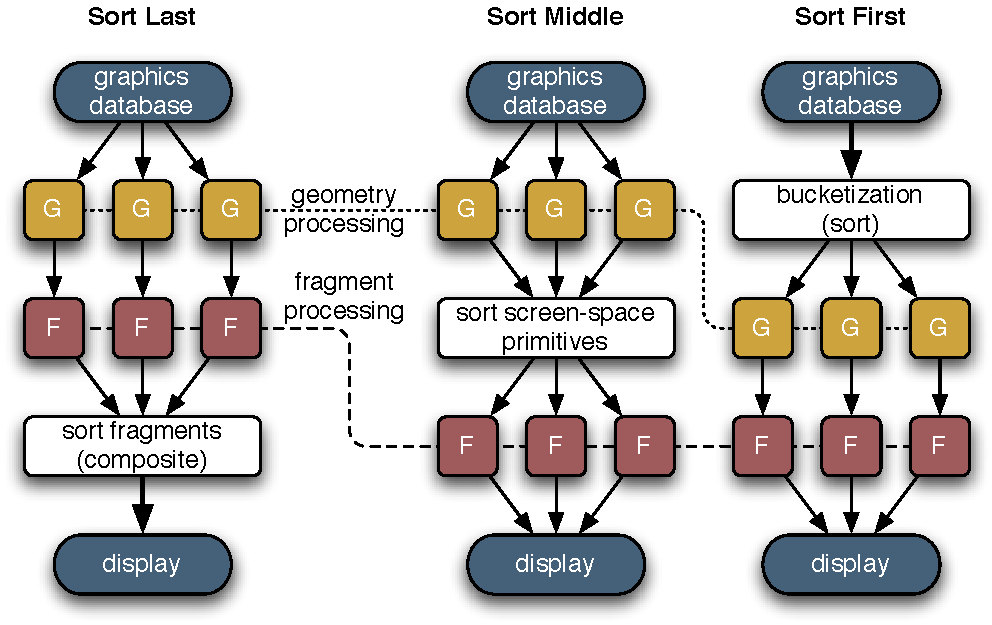
\includegraphics[width=0.7\textwidth]{images/all_sorts}%
\caption{Sort-last, sort-middle and sort-first parallel rendering\label{fSorts}}
\end{figure}


\subsection{Domain specific solutions}

Cluster-based parallel rendering has been commercialized for off-line rendering
(i.e. distributed ray-tracing) for computer generated animated movies or special
effects, since the ray-tracing technique is inherently amenable to
parallelization for off-line processing. Other special-purpose solutions exist
for parallel rendering in specific application domains such as volume rendering
\cite{LWMT:97,Wittenbrink:98,HSCSM:00,SL:02,GS:02,NSJLYZ:05} or
geo-visualization \cite{VR:91,AG:95,LDC:96,JLMV:06}. However, such specific
solutions are typically not applicable as a generic parallel rendering paradigm
and do not translate to arbitrary scientific visualization and distributed
graphics problems.

In \cite{NC:07}, parallel rendering of hierarchical level-of-detail (LOD) data
has been addressed and a solution specific to sort-first tile-based parallel
rendering has been presented. While the presented approach is not a generic
parallel rendering system, basic concepts presented in \cite{NC:07} such as load
management and adaptive LOD data traversal can be carried over to other
sort-first parallel rendering solutions.

\subsection{Special-purpose architectures}

Historically, high-performance real-time rendering systems have relied on an
integrated proprietary system architecture, such as the early SGI graphics super
computers. These special-purpose solutions have become a niche product as their
graphics performance does not keep up with off-the-shelf workstation graphics
hardware and scalability of clusters.

Due to its conceptual simplicity, a number of special-purpose image compositing
hardware solutions for sort-last parallel rendering have been developed. The
proposed hardware architectures include Sepia \cite {MHS:99a,sepia}, Sepia~2
\cite{LMSBHa:01,LMSBH:01}, Lightning~2 \cite{Stoll01}, Metabuffer
\cite{Blanke00,Zhang01}, MPC Compositor \cite{Muraki01} and PixelFlow
\cite{Molnar92, Eyles97}, of which only a few have reached the commercial
product stage (i.e. Sepia~2 and MPC Compositor). However, the inherent
inflexibility and setup overhead have limited their distribution and application
support. Moreover, with the recent advances in the speed of CPU-GPU interfaces,
such as PCI Express, NVLink and other modern interconnects, combinations of
software and GPU-based solutions offer more flexibility at comparable
performance.

\subsection{Generic approaches}

A number of algorithms and systems for parallel rendering have been developed in
the past. On one hand, some general concepts applicable to cluster parallel
rendering have been presented in \cite{Mueller:95,Mueller:97} (sort-first
architecture), \cite{SZFLS:99,SFLS:00} (load balancing), \cite{SFL:01} (data
replication), or \cite{CMF:05,CM:06} (scalability). On the other hand, specific
algorithms have been developed for cluster based rendering and compositing such
as \cite{AP:98}, \cite{CKS:02} and \cite{YYC:01,SMLAP:03}. However, these
approaches do not constitute APIs and libraries that can readily be integrated
into existing visualization applications, although the issue of the design of a
parallel graphics interface has been addressed in \cite{Igehy98}.

Only few generic APIs and (cluster-)parallel rendering systems exist which
include VR Juggler \cite{BJHMBC:01} (and its derivatives), Chromium
\cite{HHNFAKK:02} (an evolution of \cite{Humphreys99,Humphreys00,HEBSEH:01}),
{ClusterGL}~\cite{NHM:11} and OpenGL Multipipe SDK
\cite{JDBJBCER:04,BRE:05,MPK}. These approaches can be categorized into
transparent interception and distribution of the OpenGL command stream and into
the parallization of the application rendering code (\fig{fChromium}).

\begin{figure}[ht]
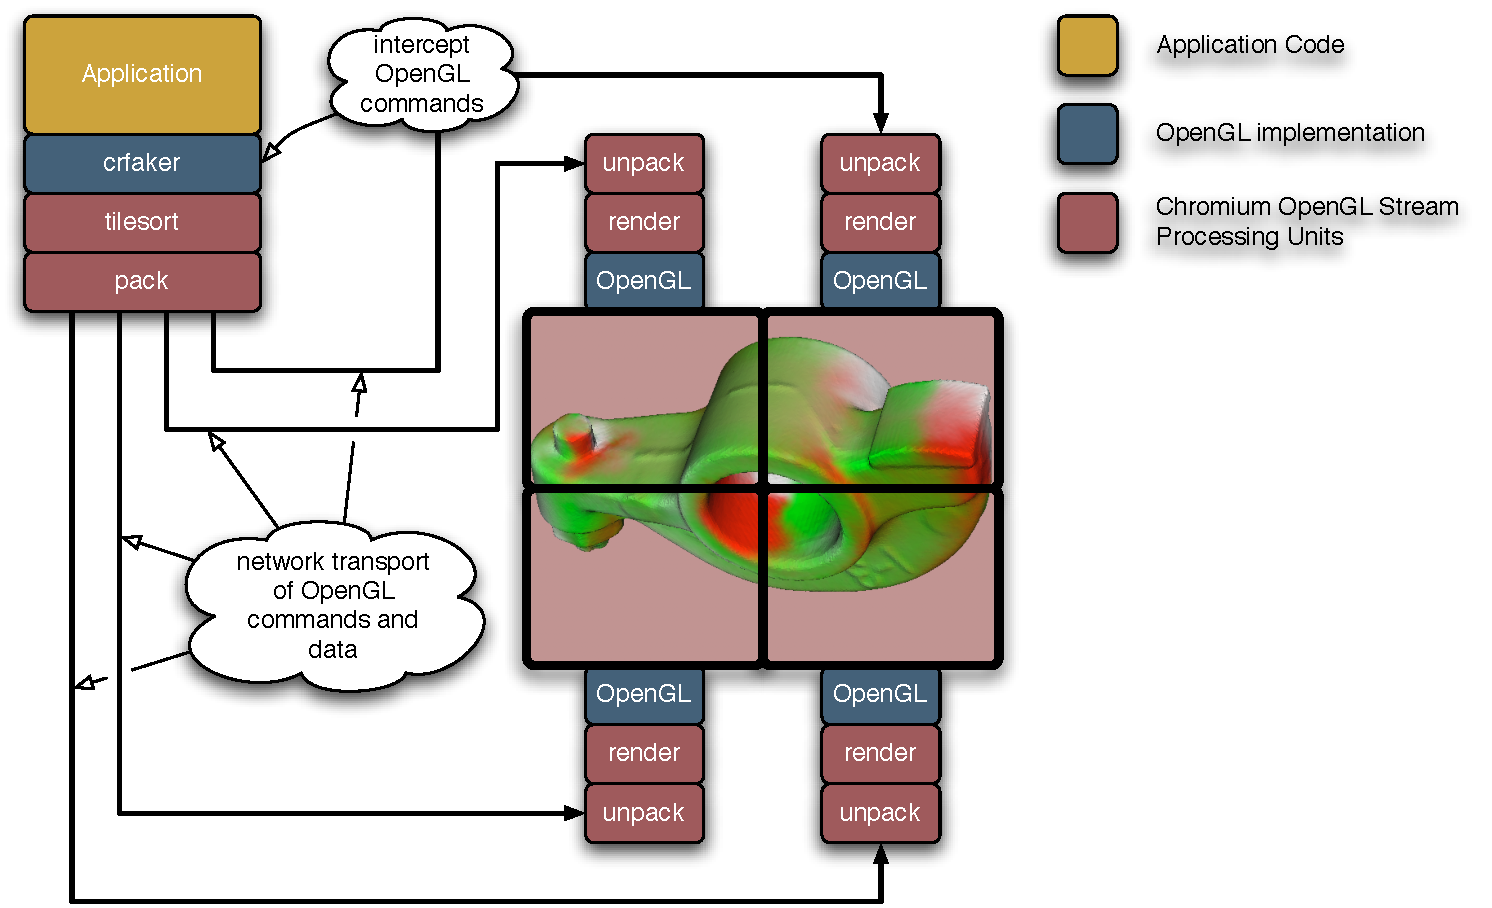
\includegraphics[height=4cm]{images/Chromium}\hfil%
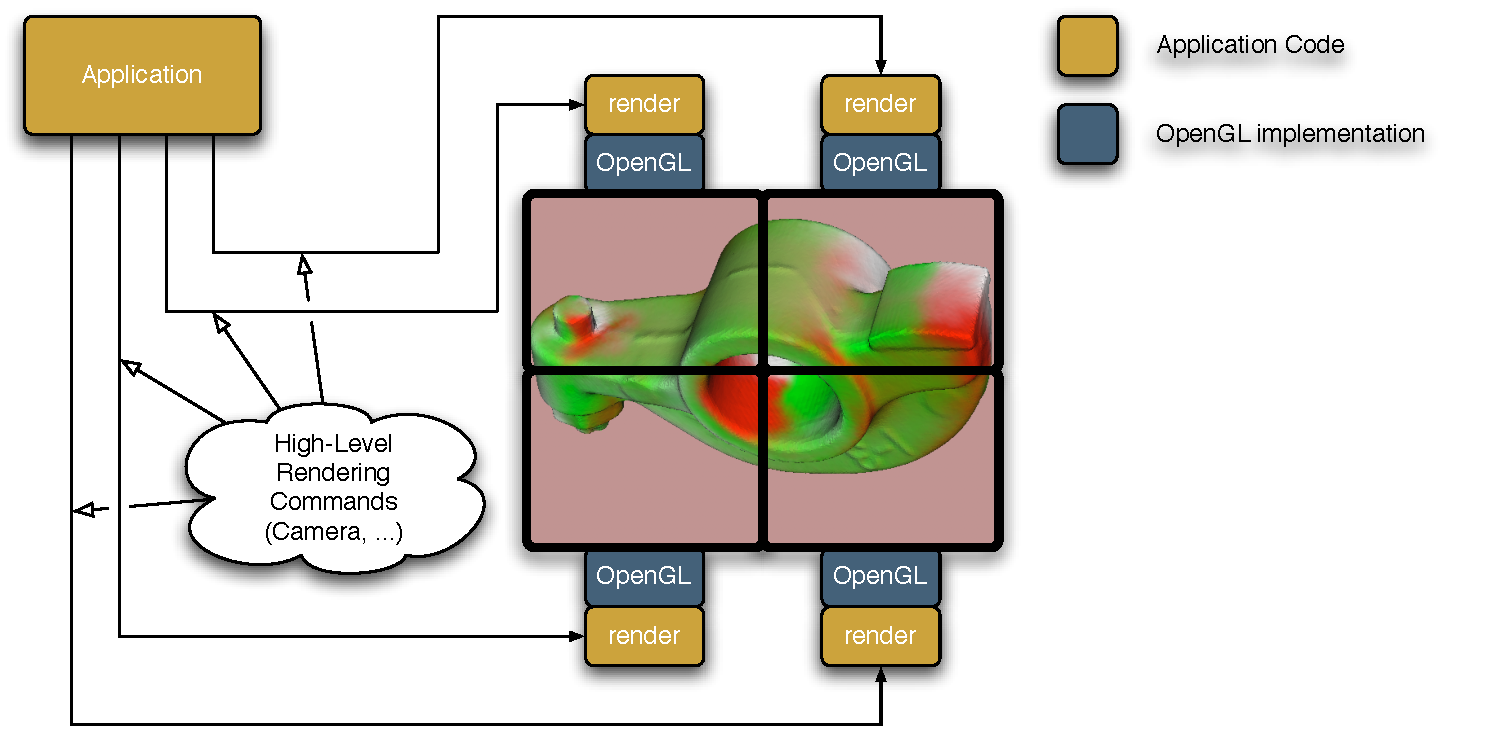
\includegraphics[height=4cm]{images/MPK}%
\caption{Transparent OpenGL interception and parallelization of the rendering code\label{fChromium}}
\end{figure}


VR Juggler \cite{BJHMBC:01,JBBC:98} is a graphics framework for virtual reality
applications which shields the application developer from the underlying
hardware architecture, devices and operating system. Its main aim is to make
virtual reality configurations easy to set up and use without the need to know
details about the devices and hardware configuration, but not specifically to
provide scalable parallel rendering. Extensions of VR Juggler, such as for
example ClusterJuggler \cite{BC:03} and NetJuggler \cite{AGLMR:02}, are
typically based on the replication of application and data on each cluster node
and basically take care of synchronization issues, but fail to provide a
flexible and powerful configuration mechanism that efficiently supports scalable
rendering as also noted in \cite{SWNH:03}. VR Juggler does not support scalable
parallel rendering such as sort-first and sort-last task decomposition and image
compositing nor does it provide support for network swap barriers
(synchronization), distributed objects, image compression and transmission, or
multiple rendering threads per process, important for multi-GPU systems.

While Chromium \cite{HHNFAKK:02} provides a powerful and transparent abstraction
of the OpenGL API, that allows a flexible configuration of display resources,
its main limitation with respect to scalable rendering is that it is focused on
streaming OpenGL commands through a network of nodes, often initiated from a
single source. This has also been observed in \cite{SWNH:03}. The problem comes
in when the OpenGL stream is large in size, due to not only containing OpenGL
calls but also the rendered data such as geometry and image data. Only if the
geometry and textures are mostly static and can be kept in GPU memory on the
graphics card, no significant bottleneck can be expected as then the OpenGL
stream is composed of a relatively small number of rendering instructions.
However, as it is typical in real-world visualization applications, display and
object settings are interactively manipulated, data and parameters may change
dynamically, and large data sets do not fit statically in GPU memory but are
often dynamically loaded from out-of-core and/or multiresolution data
structures. This can lead to frequent updates not only of commands and
parameters wich have to be distributed but also of the rendered data itself
(geometry and texture), thus causing the OpenGL stream to expand dramatically.
Furthermore, this stream of function calls and data must be packaged and
broadcast in real-time over the network to multiple nodes for each rendered
frame. This makes CPU performance and network bandwidth a more likely limiting
factor.

The performance experiments in \cite{HHNFAKK:02} indicate that Chromium is
working quite well when the rendering problem is fill-rate limited. This is due
to the fact that the OpenGL commands and a non-critical amount of rendering data
can be distributed to multiple nodes without significant problems and since the
critical fill-rate work is then performed locally on the graphics hardware.

Chromium also provides some facilities for parallel application development,
namely a sort-last, binary-swap compositing SPU and an OpenGL extension
providing synchronization primitives, such as a barrier and semaphore. It leaves
other problems, such as configuration, task decomposition as well as process and
thread management unaddressed. Parallel Chromium applications tend to be written
for one specific parallel rendering use case, such as for example the sort-first
distributed memory volume renderer \cite{BHPB:03} or the sort-last parallel
volume renderer raptor \cite{Raptor}. We are not aware of a generic
Chromium-based application using many-to-one sort-first or stereo
decompositions.

The concept of transparent OpenGL interception popularized by WireGL and
Chromium has received some further contributions. While some commercial
implementations such as {TechViz} and {MechDyne Conduit} continue to exist, on
the research side only {ClusterGL}~\cite{NHM:11} has been presented recently.
{ClusterGL} employs the same approach as {Chromium}, but delivers a
significantly faster implementation of transparent OpenGL interception and
distribution for parallel rendering. Transparent OpenGL interception is an
appealing apporach for some applications since it requires no code changes, but
it has inherent limitiations due to the fact that eventually the bottleneck
becomes the single-threaded application rendering code, the amount of
application data the single application instance can load or process, or the the
size of the OpenGL command stream send over the network.

{CGLX}~\cite{DK:11} tries to bring parallel execution transparently to
OpenGL applications, by emulating the GLUT API and intercepting certain OpenGL
calls. In contrast to frameworks like {Chromium} and {ClusterGL}
which distribute OpenGL calls, {CGLX} follows the distributed application
approach. This works transparently for trivial applications, but quickly
requires the application developer to address the complexities of a distributed
application, when mutable application state needs to be synchronized across
processes. For realistic applications, writing parallel applications remains the
only viable approach for scalable parallel rendering, as shown by the success of
{Paraview}, {Visit} and {Equalizer}-based applications.

OpenGL Multipipe SDK (MPK) \cite{BRE:05} implemented an effective parallel
rendering API for a shared memory multi-CPU/GPU system. It is similar to IRIS
Performer \cite{RH:94} in that it handles multi-GPU rendering by a lean
abstraction layer via a conceptual callback mechanism, and that it runs
different application tasks in parallel. However, MPK is not designed nor meant
for rendering nodes separated by a network. MPK focuses on providing a parallel
rendering framework for a single application, parts of which are run in parallel
on multiple rendering channels, such as the culling, rendering and final image
compositing processes.

Software for driving and interacting with tiled display walls has received
significant attention, including {Sage}~\cite{Sage} and
{Sage~2}~\cite{Sage2} in particular. {Sage} was built entirely
around the concept of a shared framebuffer where all content windows are
separate applications using pixel streaming but is no longer actively supported.
{Sage 2} is a complete, browser-centric reimplementation where each
application is a web application distributed across browser instances.
{DisplayCluster}~\cite{DisplayCluster}, and its continuation
{Tide}~\cite{tide}, also implement the shared framebuffer concept of
{Sage}, but provide a few native content applications integrated into the
display servers. These solutions implement a scalable display environment and
are a target display platform for scalable 3D graphics applications.

\section{Problem Statement}

Visualization of large amounts of data has been always been encumbered by
sufficient system software. Compared to other domains, such as HPC simulations,
large data visualization has received relatively little attention in both
research and development. Consequently, there is a large amount of data which
has not been explored sufficiently. In particular in scientific visualization,
where data is often spatial and temporal, even simple visualizations can extract
new information and provide a valuable tool to domain scientists for discovery.

The central theme of the proposed research is therefore: {\bf How can we improve
the capabilities of existing visualization algorithms for rendering large
amounts of data?} This generic problem can be researched more concretely along
the following research questions:
\begin{compactenum}
\item How can we improve the rendering performance of visualization applications to enable users to explore more data?
    \begin{compactenum}
    \item What new algorithms will decrease the time needed to composite rendering results, in particular for sort-last rendering?
    \item How can we improve load-balancing for sort-first rendering, in particular for large display systems?
    \end{compactenum}
\item How can we reduce end-to-end system latency for better user experience?
    \begin{compactenum}
    \item In a generic parallel rendering framework, how can we schedule the different rendering stages to minimize the latency for the user?
    \item How can we architect the parallel rendering framework to minimize synchronization between threads?
    \end{compactenum}
\item How can we maximize the impact of this research on large data scientists?
\end{compactenum}

The obvious solution to the problem is to utilize more compute resources to
parallelize and scale the rendering algorithm. The goal can either be to
increase strong scaling (render a given data set faster) or weak scaling (render
a larger data set at roughly the same speed). To efficiently use more resources,
we need to research increasing the parallelism of existing algorithms, and to
reduce the bottleneck in the image compositing stage.

An important collateral problem is the overall latency of the rendering system,
that is, the time between a user input and its resulting output frame. While
this is lower-bounded by the framerate of the rendering, oftentimes algorithmic
or implementation choices increase the total system latency. Often this is a
side effect of improving the rendering performance, but it also decreases the
usability of the application for interactive usage. One typical example is
pipelining of operations in the rendering pipeline.

Visualizing large amounts of data often goes hand in hand with the usage of
high-resolution displays. Since large amounts of data tends to have a lot of
detail, high-resolution desktop screens (4K or 8K resolution), as well as
high-resolution display walls, help tremenduously in recognising and
understanding details of the data. The high resolution however aggravetes all
the aforementioned problems: The increased pixel count reduces rendering
performance, requires better compositing algorithms, and increases the latency
due to longer transfer times during compositing and display. Since pixel count
increases quadratically with display size, this problem will become more
important as display resolution increases.

\section{Proposed Solution} % 2-6

Parallel rendering has received a lot of attention in the last couple of
decades, yet libraries and frameworks to develop parallel rendering applications
are scarcely available. Consequently, there are only a few applications which
can utilize parallelism for rendering, let alone do so efficiently at scale.
This research proposes to address these shortcomings by developing {\bf reusable
software components} to make parallel rendering programs easier to develop, by
generalizing existing research into reusable software implementations.

Based on these foundations, we propose to research new algorithms to improve
rendering performance. In particular we see potential in improving the
scalability through better {\bf load balancing}, {\bf image compositing}
algorithms, and {\bf holistic optimization} of the whole rendering pipeline
under control of our framework. Orthogonally to this algorithmic research, we
propose to research {\bf data processing and data access} strategies for
parallel rendering applications. This is particularly important, yet
underdeveloped, in the context of the visual analysis for HPC simulation
results.

Previous parallel rendering approaches typically failed in one of the following
system requirements:
%
\begin{compactenum}
\item generic application support, instead of domain-specific solution
\item scalable abstraction of the graphics layer
\item exploit existing code infrastructure, such as proprietary scene graphs, molecular data structures, level-of-detail and geometry databases
\end{compactenum}

To date, generic and scalable parallel rendering frameworks that can be adopted
to a wide range of scientific visualization domains are not yet readily
available. Furthermore, flexible configurability to arbitrary cluster and
multi-display configurations has also not been addressed in the past, but is of
immense practical importance to scientists depending on high-performance
interactive visualization as a scientific tool. We propose a novel flexible
framework for parallel rendering that supports scalable performance,
configuration flexibility, is minimally invasive with respect to adapting
existing visualization applications, and is applicable to virtually any
scientific visualization application domain.

To that end, this work aims to significantly advance the system design and
implementation of flexible, distributed and cluster-parallel rendering
frameworks as well as algorithms and system design for large data processing in
the context of interactive visualization. The core of this proposal is the
Equalizer project, a foundation for scalable, multi-GPU visualization software
in all application domains. The main contributions of such a parallel rendering
system are:
%
\begin{compactenum}
\item novel concept for flexible runtime configuration of graphics system resources
\item easy specification of parallel task decomposition and image compositing algorithms
\item automatic decomposition and distributed execution of rendering tasks according to the configuration
\item support for polygonal and volume rendering for opaque and transparent geometries
\item fully decentralized software architecture providing network swap barrier synchronization and data distribution functionality
\item support for low-latency distributed frame synchronization and image compositing
\item minimally invasive programming model
\end{compactenum}

The broader impact of this work revolves around the development and improvement
of a generic, flexible and scalable parallel rendering infrastructure applicable
to a large number of application domains. The expected improvements of the
proposed activities in distributed parallel parallel rendering will be
integrated into open source software libraries and as such will be available to
the general public and especially to developers of high-performance
visualization and interactive rendering applications. This approach will
maximize the impact of this research on large data scientists (research question
4).

A strong focus during the development is to architect the framework for
scalability to address research questions 1 and 2. Based on my previous work and
the study of existing implementations, scalability in parallel rendering today
is mostly limited by excessive synchronization between execution threads,
imbalance in the task decomposition, and compositing performance. Equalizer only
has the following necessary synchronization points:
%
\begin{compactenum}
\item Swap synchronization between output channels to the same display system
\item Finalization of rendering frames given a configurable latency for all render threads
\item Availability of image data for compositing between the source and destination threads
\end{compactenum}
%
This architecture has proven to provide good scalability by inherently allowing
the pipelining of data synchronization, rendering and compositing tasks
(research question 1), while simultaneously minimizing the time to display
results by letting render threads execute as early as possible (research
question 2). Furthermore, this will provide better scalability for the more
specific research questions 1(a) and 1(b).

The following publications are planned or already published to address the corresponding research question:
\begin{compactenum}
    \item
    \begin{compactenum}
        \item In \cite{EP:07, MEP:10, EBAHMP:12} we presented different algorithms to optimize the compositing step for sort-last rendering and optimisations for modern multi-GPU NUMA nodes.
        \item In \cite{EEP:11, SPEP:16} we presented novel load-balancing algorithms for sort-first rendering.
    \end{compactenum}
    \item Our first system paper \cite{EMP:09} introduces the architecture of a parallel rendering framework with minimal synchronization and optimized task scheduling, including an in-depth experimental analysis. \cite{EBAHMP:12} introduced further scheduling optimizations.
    \item Our foundation systems paper \cite{EMP:09} and applications work \cite{HBBES:13} provide evidence on the sustainability of our approach. We submitted a follow-on systems paper to ACM Transactions on Visualization and Graphics \cite{ESP:18}. This paper also contains background on applications and integrations of Equalizer in other software packages.
\end{compactenum}

Based on this generic parallel rendering framework, we propose to research
concrete algorithms and applications. We propose an engineering-driven approach
which will analyse existing algorithms, improve them incrementally by focusing
on one aspect of a large data application, and then compare our new research
against existing work. Since our research questions are largely performance
related, this comparison will be in most cases performed through benchmarking.
In particular, we see potential in:
%
\begin{compactdesc}
\item [Load-balancing for rendering resources:] While basic algorithms have been
proposed for reactive and proactive load-balancing of simple rendering tasks,
research is still needed for improving the resource utilisation for large-scale
parallelization, as well as for rendering in more complex multi-display
environments such as tiled display walls and immersive installations. The
results of this research is directly measurable through application benchmarking
of representative data sets. We consider this research goal achieved if we
proposed and implemented new algorithms which can consistently deliver better
performance over existing work, addressing research question 1(b).
\item [Compositing of the rendering results:] Previous research has focused on
the scalability for very large scale HPC runs in the order of hundreds of
thousands of cores, which are oftentimes not interactive by nature. We propose
to improve image compositing performance for interactive applications on
medium-sized (up to hundreds of GPUs) visualization clusters through analysing
and optimising image compositing algorithms. As with load-balancing, this area
of research can be considered achieved if benchmarks show consistent improvement
over state of the art algorithms, addressing research question 1(a).
\item [Applications for parallel rendering:] While a few parallel rendering
applications exist, developing them is still a significant undertaking. We
propose to extend existing rendering applications and algorithms for scientific
visualization for parallel rendering. Not only will this create new results and
capabilites for large data visualization, it also improves the general
applicability and ease of use of our generic parallel rendering components. We
consider this goal achieved if our framework is used in multiple visualization
applications. A side effect of this goal is addressing research question 4.
\item [Data management for visualization of HPC data:] We see a substantial
potential in combining big data management strategies from the cloud computing
domain to processing and visualising HPC simulation data. Paradoxically, storage
systems for HPC are often optimised for large, sequential access, which is
predominant during write, but not typical for analysis and visualization which
use more, but smaller scattered read accesses. This is an exploratory research
goal, where we hope to demonstrate the usefulness of cloud computing storage
systems for HPC storage and linked large data visualizations. We consider this
goal reached if we evaluated multiple approaches to data storage against their
traditional parallel filesystem implementation, and can make recommendations for
future research. The evaluation will again be benchmark-based, by measuring the
time to solution for typical data access patterns.
\end{compactdesc}

This research will have a sustainable impact on how we use large-scale
visualization systems as their commoditization makes them affordable to many
more organizations. This is due to the research approach of using an
incremental, engineering-driven and data-validated strategy, open source
implementation of most software artefacts, the development of high-quality
foundations, as well as the collaboration with both research and industry
partners during the research.

The proposed research will have a direct, significant impact on accelerating the
simulation-based research performed in the Blue Brain Project. On one hand, the
data distribution capabilities will allow faster development of scalable,
neuroscience-specific visualization applications for the BBP. This is of
particular importance as we foresee the need to visualize different modalities
at different brain scales as the simulations grow in complexity and data size in
the future.

\section{Research Plan\label{sPlan}}

The proposed research is heavily based on prior software engineering work in the
domain, and will leverage a strong parallel rendering system to enable novel
research within a non-trivial software stack. Consequently, a large portion of
the plan is the development of the parallel rendering framework, where the
timeline has been reverse-engineered from the work performed leading to this
proposal.

The integration of these frameworks into applications is not part of this
research schedule, since it is a non-research activity. These developments have
been and will be funded by other means. This work is nevertheless an important
part of this project, as it validates the general applicability of this research
in academia and industry.
\clearpage
The research is structured as follows:
%
\begin{compactdesc}
\item[M1-3: System Architecture:] Outline the general system architecture,
configuration structure and entities, class hierarchy and API. Research
third-party technologies to be used in the implementation.
\item[M4-10: Distributed Execution Layer:] First iteration of the implementation
of the distributed execution layer allowing dynamic configurations and
communication patterns.
\item[M10-16: Multi-Display Parallel Rendering Framework:] Based on the
distributed execution layer, develop a first parallel rendering framework
capable of driving multi-display environments for monoscopic rendering,
including the automatic launch of the rendering processes from the main
application.
\item[M17: Stereoscopic Rendering:] Implement stereoscopic rendering using
configurable interocular distance.
\item[M18: Immersive Rendering:] Head-tracking API and configuration entities,
calculation of corresponding off-axis frusta.
\item[M19: Scalable Rendering Architecture:] Design configuration and class
hierarchy for scalable rendering modes, including task decomposition and
parallel compositing algorithms.
\item[M20-24: Basic Scalable Rendering:] Implement basic decompositions (2D, DB,
Eye) and corresponding parallel compositing algorithms (2D, direct-send,
binary-swap).
\item[M25-30: Advanced Scalable Rendering:] Implement advanced compounds (Pixel,
DPlex) and compositing optimizations (realtime image compression, region of
interest, etc.).
\item[M30-32: First Publication:] Benchmarking and systems paper.
\item[M33-36: Load Balancing:] Implement load-balancing for multi-display
setups. improved automatic load-balancing using region of interest.
\item[M37-38: Second Publication:] Benchmarking and load-balancing paper.
\item[M39-42: Compositing Research:] Research compositing optimizations.
\item[M43-44: Third Publication:] Benchmarking and compositing paper.
\item[PhD Proposal]
\item[M45-46: Fourth Publication:] Benchmarking and updated systems paper.
\item[M47-52: Dissertation:] Write and defend dissertation.
\end{compactdesc}

\appendix
\section{Reviewer Comments}

In the following we quote the comments from the oral defense, and how they have
been addressed in this revised proposal.

\begin{displayquote} The core part of the proposal should explain in detail how
you want to address the research questions. This is missing. While four research
questions are stated in section 3 (Problem Statement) these are not revisited in
Section 4 (Proposed Solution). It remains unclear how exactly you want to
approach your research questions and how you want to evaluate your solutions.

Section 4 is too short. Discuss each research question in turn and state the
expected outcomes (e.g., deadline and venue to which you have planned to submit
a paper; tentative title of paper).

A research plan should be added.
\end{displayquote}

Section 4 now contains back-references to the research questions, as well as a
list of planned and accepted publications. A new Section 5 contains the research
plan.


\begin{displayquote} Although the aim to create a “generic parallel rendering
system” is commendable. I would recommend having the initial scope of the system
clearly defined. For example, describing a set of (1) the data characteristics
and (2) the interactive tasks that the system will initially support. Having
this clear scope would allow the author to know when to stop broadening the
support of the system and start addressing other goals of the thesis.
\end{displayquote}

The proposal does not clearly show the history and context since it would incur
too much software engineering context: The generic parallel rendering system is
developed, with a clearly defined scope and roadmap based on previous work. The
added \sref{sPlan} shows the effective timeline, where your concern would be
covered by month 1 to month 30. Furthermore, a substantial part of the
implementation needed for the fourth publication was supported by commercial
activities.

\begin{displayquote} As the author pointed out the latency from “data
processing” may slow down users’ workflow  during interactive exploration.
While the author develops the rendering system, what would be the strategy to
prevent the influence of (currently inefficient) data processing? For example,
when the author tests the rendering system on a large cluster of GPU with a
large amount of data, how would he be able to distinguish the latency of
rendering from the latency of data processing? How would such strategy ensure
ecological validity (i.e., the test setting is representative to how the
rendering system will be actually used)?
\end{displayquote}

For research, these two components can often be decoupled for evaluating one
aspect of the system. For example, a parallel compositing algorithm can be
optimised and benchmarked on synthetic data which has no significant data
processing. Likewise, an improved data loading can be optimised against its
traditional implementation while keeping the parallel rendering configuration
(decomposition, load-balancing, and compositing) constant. If desired, a whole
system evaluation can be evaluated against the time-to solution, for example by
benchmarking the time needed to perform a recorded navigation against a baseline
implementation and any variation of new parallel rendering and data processing
algorithms. This would closely mirror the user experience, which is governed by
the reactiveness of the application.

During the review of the proposal we realized that the data processing component
should not be part of this proposal, since it represents an orthogonal research
question, and should be kept separate to avoid confusion.

\begin{displayquote} To address contribution “2. easy specification…” and “7.
minimally invasive programming model”, the author proposed porting current
science via applications onto the proposed rendering system. I agree that this
will validate the “applicability”, it falls short at validating the “ease of
use” of the API. I would suggest to work closely with other software developers
in the Blue Brain project and observe how they use the API of the rendering
system. Use their feedback to iteratively improve the API. In the final version
of the API, observe how long these developers take to learn the rendering system
until they successfully port their application.
\end{displayquote}

Since this proposal is research-oriented it does not address this concern. In
reality, the API has been developed based on experience and developer feedback
with OpenGL Multipipe SDK, as well as during the development of the Equalizer
parallel rendering framework, open source community engagement, commercial
consulting activities, and work at the Blue Brain Project. Below are some
quotations from these activities:

\begin{compactdesc}
\item[September 2012, Alessandro Febretti, Ph.D. Student, EVL, University of Illinois at Chicago:] I have been working with Equalizer for more than a year now and overall it has been a fantastic experience. Equalizer simplified my development work a whole lot.
\item[February 2009, Brian Gianforcarom, Computer Science at Rochester Institute of Technology:] I've worked on projects trying to do similar things without Equalizer, and I can honestly say it was pretty bad. We only got it barely working. After finding Equalizer later, I can't imagine how much easier it would have been with such a tool.
\item[November 2008, Dan Wilcox, developer at Ars Electronica Futurelab:] Equalizer abstracts the windowing and distribution of shared objects which, trust me, is well worth the overhead of learning it. It's one thing to have each machine running the same rendering thread and it's quite another to send control and input dynamically between them. Plus it runs on Mac, Windows, and Linux. (source)
\item[April 2008, Nicolas Cuntz, researcher at the University of Siegen:]Equalizer bundles multi-node rendering and synchronization tools into an easy-to-use and well-structured object-oriented framework. Porting to Equalizer can be achieved without completely restructuring the application. However, one has to deal with data synchronization and possible problems related to threading and parallelism, which is a problem that cannot completely be delegated to a library.
\end{compactdesc}

\begin{displayquote} It is unclear which stage of the PhD study the author is
currently at, and how does the previous work of the author fit into this
proposal. For example, is the Equalizer project a part of the PhD study? What
papers from the PhD work are published and what are planned?
\end{displayquote}

The new \sref{sPlan} has a marker for the current state at the PhD proposal. We
plan to publish an updated systems paper on Equalizer and a publication of
parallel rendering for out-of-core volume rendering. Published and relevant for
the dissertation are \cite{EMP:09, EEP:11, EP:07, HBBES:13, EBAHMP:12, MEP:10}
as well as unpublished work in the context of key-value storage and
visualization web services.

\begin{displayquote} The claim of “sustainable” parallel rendering framework
needs clear specification and evaluation criteria. In particular, how would you
know that your implementation covers necessary and sufficient building blocks
for further research/development on parallel implementation? (See point 1,
above.)
\end{displayquote}

This is arguably a soft criteria, which has some needed but not necessarily sufficient requirements:
\begin{compactitem}
\item Open Source implementation and community
\item Successful porting of different types of applications to Equalizer
\item Other independent research based on Equalizer
\end{compactitem}

So far, we have worked with different applications for large volume rendering,
scientific visualization, as well as commercial application for high-quality
design renderings. Equalizer is maintained on github, and has attracted
third-party research both in Prof. Pajarola's lab \cite{GMBP:10, EBAHMP:12,
MEP:10, GEMPG:13} and externally \cite{Omegalib, FNTTL:13}.

\begin{displayquote} The performance evaluation (point 2, above) is further
compounded by the introduction of supports for cloud data storage, which will
further impose latency in “data processing” step. I would suggest describing
clear evaluation strategies.
\end{displayquote}

Correct, some of this is addressed above. My working hypothesis is that
key-value stores can actually decrease the latency over HPC-style parallel file
systems for visualization workloads. Visualization workload tends to have more
random access of smaller data items from a few processes, whereas parallel file
systems tend to be optimized for large sequential operations from a large amount
of processes. Some preliminary work in this direction has been published in
\cite{Eilemann:15}. As mentioned above, we have decided to omit this part from
the revised proposal.


\begin{displayquote}
\end{displayquote}

\begin{displayquote}
\end{displayquote}


\clearpage
\bibliographystyle{alpha}
\bibliography{references/references}
% Add your glossary here
% Add your index here

\end{document}
